\documentclass[../../../main.tex]{subfiles}
\begin{document}

%%%%%%%%%%%%%%%%%%%%%%%%%%%%%%%%%%%%%%%%%
%%%%%%%%%%%%%%%%%%%%%%%%%%%%%%%%%%%%%%%%%
%%%%%%%%%%%%%%%%%%%%%%%%%%%%%%%%%%%%%%%%%
\chapter{One and two tailed tests}

There are three kinds of hypothesis tests that we can make with a single sample:

\begin{itemize}
  \item Left-tailed test
  \item Right-tailed test
  \item Two-tailed test
\end{itemize}

\noindent
The first two are one-tailed tests. The difference between them is whether we care about the tail on the left side of the curve, or the right side of the curve. For two-tailed tests, we care about both sides of the curve.


%%%%%%%%%%%%%%%%%%%%%%%%%%%%%%%%%%%%%%%%%
%%%%%%%%%%%%%%%%%%%%%%%%%%%%%%%%%%%%%%%%%
\section{One tailed tests (left tail)}

We discussed an example of a left tailed test already, in the example of McCallister Logistics. For that, we formulated these hypothesis:

\begin{align*}
  \NullHyp/: \populationmean \geq 55K \\
  \AltHyp/: \populationmean < 55K
\end{align*}

\noindent
Here we state this with the number 55K in there, but if we swap that out and put $\HypPopMean/$ in its place, we get this:

\begin{align*}
  \NullHyp/: \populationmean \geq \HypPopMean/ \\
  \AltHyp/: \populationmean < \HypPopMean/
\end{align*}

\noindent
This is the shape of $\NullHyp/$ and $\AltHyp/$ for a \vocab{left-tailed} hypothesis test. Any left-tailed test will have its $\NullHyp/$ and $\AltHyp/$ hypotheses in this exact format. (Hint: you can remember that this is a \emph{left}-tailed test because the wedge in the alternative hypothesis points to the \emph{left}.)

Why is this left-tailed? Well, the null hypothesis claims that the true population mean is greater than or equal to the hypothesized population mean. So the hypothesized population mean $\HypPopMean/$ serves as a kind of \emph{bottom limit}, or a \emph{far left-limit}, for the test. Why? If the true population mean is \emph{below} (i.e., to the \emph{left} of) the hypothesized mean, then the alternative hypothesis is true. Hence, the wedge (the less-than symbol) points to the left in $\AltHyp/$ above.

Another reason we call this a \emph{left}-tailed test is that, when we plot the hypothesized sampling distribution, we only care about $\alpha$ on the \emph{left} side of the curve. Recall the McCallister Logistics example. The hypothesized sampling distribution is centered at 55K:

\begin{center}
  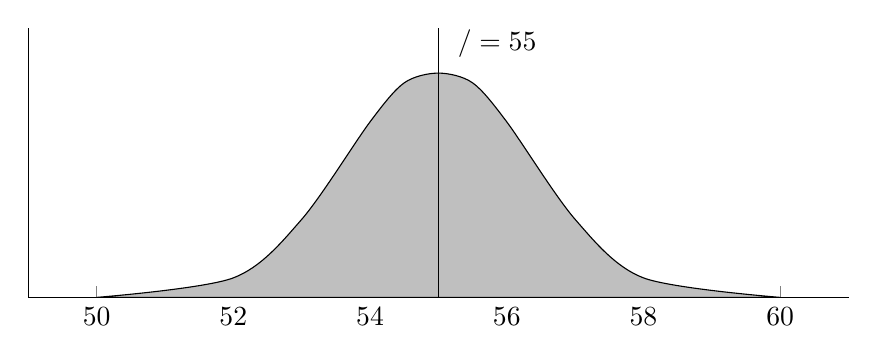
\begin{tikzpicture}
    \begin{axis}[
      axis lines*=left,
      ytick=\empty,
      height=5cm,
      width=12cm,
      enlarge y limits={value=0.2,upper},
      ]
      \addplot[smooth, fill=lightgray, domain=45:65] 
        coordinates{
          (50, 0) (52, 0.5) (53, 2) (54, 4.5) (54.5, 5.5)
          (55, 5.75)
          (55.5, 5.5) (56, 4.5) (57, 2) (58, 0.5) (60, 0)} 
        \closedcycle;

      \draw (55, 0) -- (55, 10);
      \node at (55, 6.5) [label=right:{$\HypPopMean/ = 55$}] {};

    \end{axis}
  \end{tikzpicture}
\end{center}

\noindent
As we saw before, if the true population mean is anywhere to the right of 55K, the null hypothesis stands. So we do not care what happens around the \emph{right} tail of this curve.

But we do care about what happens around the left tail of this curve. In particular, we have to draw a line in the sand by setting $\alpha$ at a particular point. For example, we can set $\alpha$ so it takes off 5\% of the total curve:

\begin{center}
  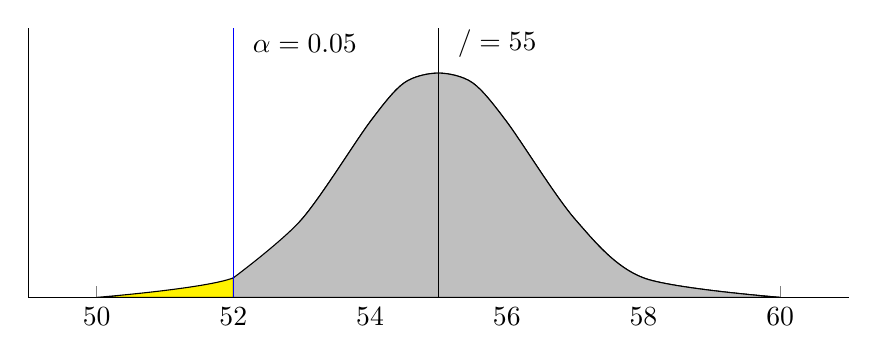
\begin{tikzpicture}
    \begin{axis}[
      axis lines*=left,
      ytick=\empty,
      height=5cm,
      width=12cm,
      enlarge y limits={value=0.2,upper},
      ]
      \addplot[smooth, fill=yellow, domain=45:65] 
        coordinates{
          (50, 0) (52, 0.5) (53, 2) (54, 4.5) (54.5, 5.5)
          (55, 5.75)
          (55.5, 5.5) (56, 4.5) (57, 2) (58, 0.5) (60, 0)} 
        \closedcycle;

      \addplot[smooth, fill=lightgray, domain=45:65] 
        coordinates{
          (52, 0.5) (53, 2) (54, 4.5) (54.5, 5.5)
          (55, 5.75)
          (55.5, 5.5) (56, 4.5) (57, 2) (58, 0.5) (60, 0)} 
        \closedcycle;

      \draw (55, 0) -- (55, 10);
      \node at (55, 6.5) [label=right:{$\HypPopMean/ = 55$}] {};

      \draw[color=blue] (52, 0) -- (52, 10);
      \node at (52, 6.5) [label=right:{$\alpha = 0.05$}] {};

    \end{axis}
  \end{tikzpicture}
\end{center}

\noindent
All of the action happens over in that left tail. The critical point $\alpha$ forms the bottom (left-most) limit for our decision procedure: we reject the null hypothesis for any sample mean that falls below (to the left of) $\alpha$. Moreover, $\alpha$ is the place where Type I errors can occur, and it is the line that determines where Type II Errors can occur too.


%%%%%%%%%%%%%%%%%%%%%%%%%%%%%%%%%%%%%%%%%
%%%%%%%%%%%%%%%%%%%%%%%%%%%%%%%%%%%%%%%%%
\section{One tailed tests (right tail)}

Right-tailed tests go the opposite direction. For example, suppose that the union claims instead that McCallister's female employees made on average \emph{more} than 55K per year. The hypotheses we would formulate would then be these:

\begin{align*}
  \NullHyp/: \populationmean \leq 55K \\
  \AltHyp/: \populationmean > 55K
\end{align*}

\noindent
And if we swap out 55K and put $\HypPopMean/$ in its place, we get this:

\begin{align*}
  \NullHyp/: \populationmean \leq \HypPopMean/ \\
  \AltHyp/: \populationmean > \HypPopMean/
\end{align*}

\noindent
This is the shape of $\NullHyp/$ and $\AltHyp/$ for a \vocab{right-tailed} hypothesis test. Any right-tailed test will have its $\NullHyp/$ and $\AltHyp/$ hypotheses in this exact format. (Hint: again, you can remember that this is a \emph{right}-tailed test because the wedge in the alternative hypothesis points to the \emph{right}.)

In this case, the null hypothesis claims that the true population mean is \emph{lower} than (or equal to) the hypothesized population mean. So here, the hypothesized population mean $\HypPopMean/$ serves as the \emph{top limit}, or the \emph{far right limit}, for the test. So, if the true population mean were \emph{above} (i.e., to the \emph{right} of) the hypothesized mean, then the alternative hypothesis would be true. Hence, the wedge (the less-than symbol) points to the right in $\AltHyp/$ above.

When we plot the hypothesized sampling distribution, we now care about $\alpha$ on the \emph{right} side of the curve. For if the true population mean is anywhere to the left of 55K, then the null hypothesis will stand. So we do not care what happens around the \emph{left} tail of this curve.

But we do care about what happens around the right tail of this curve, because we have to draw $\alpha$ over on that side. For example:

\begin{center}
  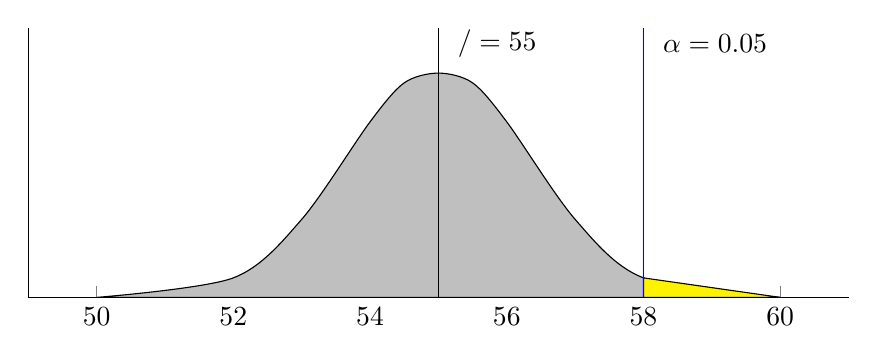
\begin{tikzpicture}
    \begin{axis}[
      axis lines*=left,
      ytick=\empty,
      height=5cm,
      width=12cm,
      enlarge y limits={value=0.2,upper},
      ]
      \addplot[smooth, fill=lightgray, domain=45:65] 
        coordinates{
          (50, 0) (52, 0.5) (53, 2) (54, 4.5) (54.5, 5.5)
          (55, 5.75)
          (55.5, 5.5) (56, 4.5) (57, 2) (58, 0.5) (60, 0)} 
        \closedcycle;

      \addplot[smooth, fill=yellow, domain=45:65] 
        coordinates{
          (58, 0.5) (60, 0)} 
        \closedcycle;

      \draw (55, 0) -- (55, 10);
      \node at (55, 6.5) [label=right:{$\HypPopMean/ = 55$}] {};

      \draw[color=blue] (58, 0) -- (58, 10);
      \node at (58, 6.5) [label=right:{$\alpha = 0.05$}] {};

    \end{axis}
  \end{tikzpicture}
\end{center}

\noindent
For this kind of a test, all of the action happens over in the right tail. The critical value $\alpha$ forms the top (right-most) limit for our decision procedure: we reject the null hypothesis for any sample mean that falls above (to the right of) $\alpha$, and Type I and Type II Errors happen on the right side, where $\alpha$ is.



%%%%%%%%%%%%%%%%%%%%%%%%%%%%%%%%%%%%%%%%%
%%%%%%%%%%%%%%%%%%%%%%%%%%%%%%%%%%%%%%%%%
\section{Two tailed tests}

Suppose that the union claims not that the average female salary is greater than or less than 55K, but rather suppose they want to say that it \emph{is} 55K. What they would be proposing is not that the true population would be above or below 55K, but rather that the true population is exactly 55K.

To formulate the null and alternative hypotheses for this, we don't use greater-than/less-than symbols. Instead, we use the equal symbol. The hypotheses we would formulate would be these:

\begin{align*}
  \NullHyp/: \populationmean = 55K \\
  \AltHyp/: \populationmean \not = 55K
\end{align*}

\noindent
Here the null hypothesis claims that the true population is exactly 55K, whereas the alternative hypothesis the opposite of that: it is the claim that the true population mean is not exactly 55K.

As before, we can swap out 55K and put $\HypPopMean/$ in its place. That gives us this pair of hypotheses:

\begin{align*}
  \NullHyp/: \populationmean = \HypPopMean/ \\
  \AltHyp/: \populationmean \not = \HypPopMean/
\end{align*}

\noindent
This is the shape of $\NullHyp/$ and $\AltHyp/$ for a \vocab{two-tailed} hypothesis test. Any two-tailed test will have its $\NullHyp/$ and $\AltHyp/$ hypotheses in this exact format.

Why is this a two-tailed test? With the one-tailed tests, we didn't care if the true population mean is higher (or lower), so there is always one side of the curve that doesn't matter. But with a two-tailed test, the null hypothesis is claiming that the true population mean is \emph{neither} above nor below the hypothesized sample mean. Hence, we have to care about both tails of the curve.

For example, here's the curve again, for the hypothesized sampling distribution centered at 55K:

\begin{center}
  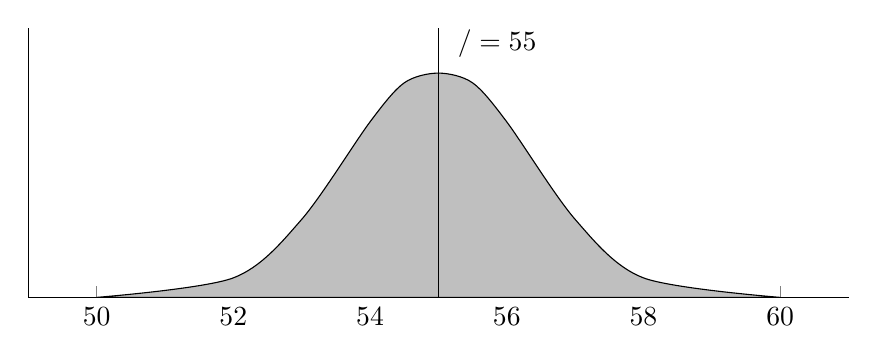
\begin{tikzpicture}
    \begin{axis}[
      axis lines*=left,
      ytick=\empty,
      height=5cm,
      width=12cm,
      enlarge y limits={value=0.2,upper},
      ]
      \addplot[smooth, fill=lightgray, domain=45:65] 
        coordinates{
          (50, 0) (52, 0.5) (53, 2) (54, 4.5) (54.5, 5.5)
          (55, 5.75)
          (55.5, 5.5) (56, 4.5) (57, 2) (58, 0.5) (60, 0)} 
        \closedcycle;

      \draw (55, 0) -- (55, 10);
      \node at (55, 6.5) [label=right:{$\HypPopMean/ = 55$}] {};

    \end{axis}
  \end{tikzpicture}
\end{center}

\noindent
If we get a sample mean that is too far to the right, then we might suspect that the true population mean is over to the right:

\begin{center}
  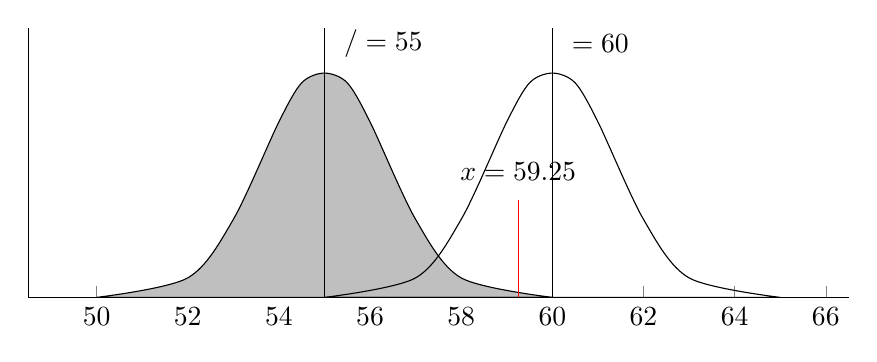
\begin{tikzpicture}
    \begin{axis}[
      axis lines*=left,
      ytick=\empty,
      height=5cm,
      width=12cm,
      enlarge y limits={value=0.2,upper},
      ]
      \addplot[smooth, fill=lightgray, domain=45:65] 
        coordinates{
          (50, 0) (52, 0.5) (53, 2) (54, 4.5) (54.5, 5.5)
          (55, 5.75)
          (55.5, 5.5) (56, 4.5) (57, 2) (58, 0.5) (60, 0)} 
        \closedcycle;

      \draw (55, 0) -- (55, 10);
      \node at (55, 6.5) [label=right:{$\HypPopMean/ = 55$}] {};

      \addplot[smooth, domain=45:65] 
        coordinates{
          (55, 0) (57, 0.5) (58, 2) (59, 4.5) (59.5, 5.5)
          (60, 5.75)
          (60.5, 5.5) (61, 4.5) (62, 2) (63, 0.5) (65, 0)} 
        \closedcycle;

      \draw (60, 0) -- (60, 10);
      \node at (60, 6.5) [label=right:{$\populationmean = 60$}] {};

      \draw[color=red] (59.25, 0) -- (59.25, 2.5);
      \node at (59.25, 2.5) [label=above:{$\samplemean{x} = 59.25$}] {};

    \end{axis}
  \end{tikzpicture}
\end{center}

\noindent
Similarly, if we get a sample that is too far to the left, then we might suspect that the true population mean is over to the left:

\begin{center}
  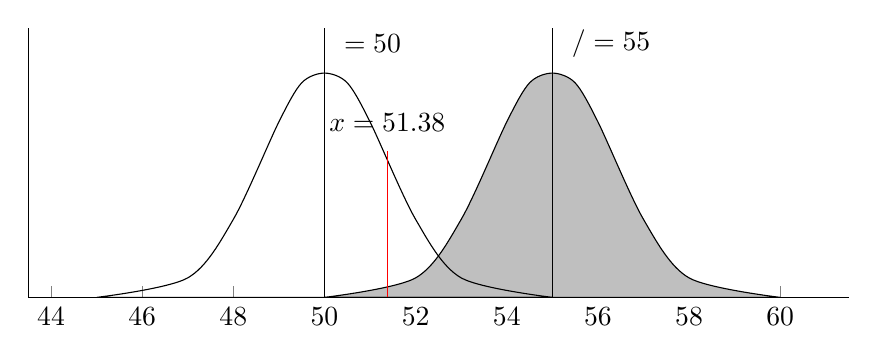
\begin{tikzpicture}
    \begin{axis}[
      axis lines*=left,
      ytick=\empty,
      height=5cm,
      width=12cm,
      enlarge y limits={value=0.2,upper},
      ]
      \addplot[smooth, fill=lightgray, domain=45:65] 
        coordinates{
          (50, 0) (52, 0.5) (53, 2) (54, 4.5) (54.5, 5.5)
          (55, 5.75)
          (55.5, 5.5) (56, 4.5) (57, 2) (58, 0.5) (60, 0)} 
        \closedcycle;

      \draw (55, 0) -- (55, 10);
      \node at (55, 6.5) [label=right:{$\HypPopMean/ = 55$}] {};

      \addplot[smooth, domain=45:65] 
        coordinates{
          (45, 0) (47, 0.5) (48, 2) (49, 4.5) (49.5, 5.5)
          (50, 5.75)
          (50.5, 5.5) (51, 4.5) (52, 2) (53, 0.5) (55, 0)} 
        \closedcycle;

      \draw (50, 0) -- (50, 10);
      \node at (50, 6.5) [label=right:{$\populationmean = 50$}] {};

      \draw[color=red] (51.38, 0) -- (51.38, 3.75);
      \node at (51.38, 3.75) [label=above:{$\samplemean{x} = 51.38$}] {};

    \end{axis}
  \end{tikzpicture}
\end{center}

\noindent
So we need to set a critical point on \emph{both} sides of the curve:

\begin{center}
  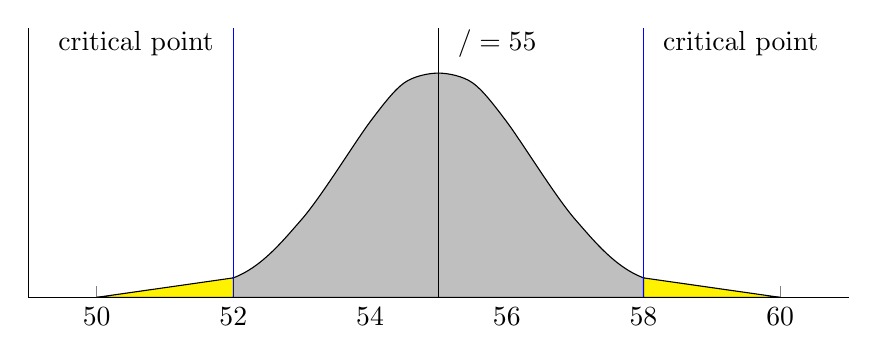
\begin{tikzpicture}
    \begin{axis}[
      axis lines*=left,
      ytick=\empty,
      height=5cm,
      width=12cm,
      enlarge y limits={value=0.2,upper},
      ]
      \addplot[smooth, fill=lightgray, domain=45:65] 
        coordinates{
          (50, 0) (52, 0.5) (53, 2) (54, 4.5) (54.5, 5.5)
          (55, 5.75)
          (55.5, 5.5) (56, 4.5) (57, 2) (58, 0.5) (60, 0)} 
        \closedcycle;
        
      \addplot[smooth, fill=yellow, domain=45:65] 
        coordinates{
          (50, 0) (52, 0.5)} 
        \closedcycle;

      \addplot[smooth, fill=yellow, domain=45:65] 
        coordinates{
          (58, 0.5) (60, 0)} 
        \closedcycle;

      \draw (55, 0) -- (55, 10);
      \node at (55, 6.5) [label=right:{$\HypPopMean/ = 55$}] {};

      \draw[color=blue] (52, 0) -- (52, 10);
      \node at (52, 6.5) [label=left:{critical point}] {};
      
      \draw[color=blue] (58, 0) -- (58, 10);
      \node at (58, 6.5) [label=right:{critical point}] {};

    \end{axis}
  \end{tikzpicture}
\end{center}

\noindent
This way, we can say that the non-rejection region is between these two lines. So, if we take a sample and the mean of that sample ends up being between those two lines, then we do not reject the null hypothesis, but if the sample mean falls outside those two lines, then we do.

Since we are adding two critical points, we take whatever amount of $\alpha$ we want to allow for the test --- 5\%, or 1\%, or whatever --- then we divide it up into two equal parts, and we put half in the left tail, and half in the right tail. For example, if we want to allow an $\alpha$ value of 5\%, we would put 2.5\% in the left tail, and 2.5\% in the right tail:

\begin{center}
  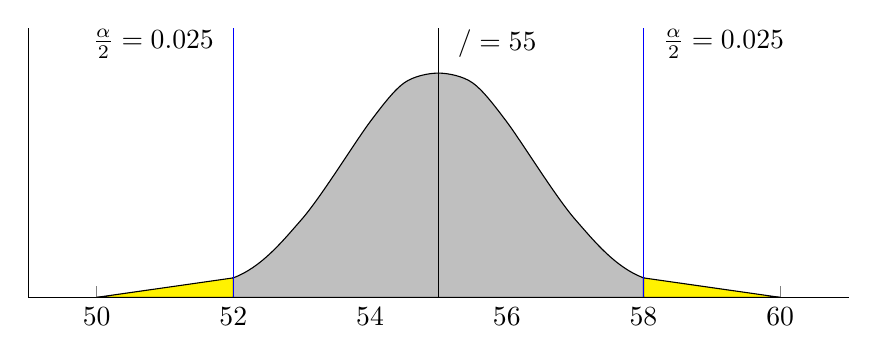
\begin{tikzpicture}
    \begin{axis}[
      axis lines*=left,
      ytick=\empty,
      height=5cm,
      width=12cm,
      enlarge y limits={value=0.2,upper},
      ]
      \addplot[smooth, fill=lightgray, domain=45:65] 
        coordinates{
          (50, 0) (52, 0.5) (53, 2) (54, 4.5) (54.5, 5.5)
          (55, 5.75)
          (55.5, 5.5) (56, 4.5) (57, 2) (58, 0.5) (60, 0)} 
        \closedcycle;
        
      \addplot[smooth, fill=yellow, domain=45:65] 
        coordinates{
          (50, 0) (52, 0.5)} 
        \closedcycle;

      \addplot[smooth, fill=yellow, domain=45:65] 
        coordinates{
          (58, 0.5) (60, 0)} 
        \closedcycle;

      \draw (55, 0) -- (55, 10);
      \node at (55, 6.5) [label=right:{$\HypPopMean/ = 55$}] {};

      \draw[color=blue] (52, 0) -- (52, 10);
      \node at (52, 6.5) [label=left:{$\frac{\alpha}{2} = 0.025$}] {};
      
      \draw[color=blue] (58, 0) -- (58, 10);
      \node at (58, 6.5) [label=right:{$\frac{\alpha}{2} = 0.025$}] {};

    \end{axis}
  \end{tikzpicture}
\end{center}

\noindent
If we set $\alpha$ to 5\% like this, we still say that the probability of Type I Error is 5\%. It's just that half of that probability lives in the left tail (where sample means can be too low), and half of that probability lives in the right tail (where sample means can be too high).


%%%%%%%%%%%%%%%%%%%%%%%%%%%%%%%%%%%%%%%%%
%%%%%%%%%%%%%%%%%%%%%%%%%%%%%%%%%%%%%%%%%
\section{The equal sign rule}

Notice that with the one and two tailed tests, there is an equal sign (or an implied equal sign) in the formulation of the hypotheses. For two tailed tests, the hypotheses are these:

\begin{align*}
  \NullHyp/: \populationmean = \HypPopMean/ \\
  \AltHyp/: \populationmean \not = \HypPopMean/
\end{align*}

\noindent
Where is the equals sign? It is the null hypothesis.

What about a left-tailed test? The hypotheses are these:

\begin{align*}
  \NullHyp/: \populationmean \geq \HypPopMean/ \\
  \AltHyp/: \populationmean < \HypPopMean/
\end{align*}

\noindent
The equals sign is in the null hypothesis again. The null hypothesis says that the true population mean is greater than \emph{or equal to} the hypothesized population mean. The alternative hypothesis has no such ``or equal to.'' It claims only that the true mean is less than the hypothesized mean.

Likewise, for a right-tailed test:

\begin{align*}
  \NullHyp/: \populationmean \leq \HypPopMean/ \\
  \AltHyp/: \populationmean > \HypPopMean/
\end{align*}

\noindent
Here too, the equal sign lives in the null hypothesis: less than \emph{or equal to}. 

The point to notice here is that the equal sign always lives in the null hypothesis, never in the alternative hypothesis. This is really just a convention. We could do it differently, but the statistics community decided (for whatever reasons) to always do it this way.


%%%%%%%%%%%%%%%%%%%%%%%%%%%%%%%%%%%%%%%%%
%%%%%%%%%%%%%%%%%%%%%%%%%%%%%%%%%%%%%%%%%
\section{Claims and implied challenges}

When we formulate the null and alternative hypotheses for a test, we treat the claims that others are making as something that we cannot believe up front, but instead as something that must be proven. 

So, we always treat someone's claim as an implied challenge, and we put it in the alternative hypothesis. Then, we formulate the null hypothesis by making it the opposite of the alternative hypothesis. Since we treat the null hypothesis as the status quo, this forces the burden of proof on the claim (in the alternative hypothesis), so the claim is not accepted without proof.

Think about how we did that with McCallister's case. When we introduced the example, we configured the null and alternative hypothesis like this:

\begin{align*}
  \NullHyp/: \populationmean \geq \HypPopMean/ \\
  \AltHyp/: \populationmean < \HypPopMean/
\end{align*}

\noindent
We treated the claim that McCallister's female employees make less than 55K a year as an implied challenge. \emph{That} is the claim that needs to be proven. So, we started with the opposite of that, namely a null hypothesis which assumes that McCallister's female employees make at least 55K per year.

\begin{align*}
  \NullHyp/: \populationmean \leq 55K \\
  \AltHyp/: \populationmean > 55K
\end{align*}

\noindent
Also, we often interpret claims as one-tailed tests, rather than two tailed tests. In other words, we assume that the mean is not as small (or as big) as the claimant says, and then we use a one-tailed test to confirm whether we have strong enough evidence to believe that it is otherwise. 

We should only use a two-tailed test if the problem at hand requires that we check that the true population mean is \emph{neither} greater \emph{nor} lesser than the hypothesized population mean.

When we formulate the hypotheses for a two-tailed test, we don't need to treat anyone's claim as an implied challenge. We also put the equals sign in the null hypothesis.

\end{document}
